\documentclass[10pt, a5paper]{article}
\usepackage{pdfpages}
\usepackage{parallel}
\usepackage[T2A]{fontenc}
\usepackage{ucs}
\usepackage[utf8x]{inputenc}
\usepackage[polish,english,russian]{babel}
\usepackage{hyperref}
\usepackage{rotating}
\usepackage[inner=2cm,top=1.8cm,outer=2cm,bottom=2.3cm,nohead]{geometry}
\usepackage{listings}
\usepackage{graphicx}
\usepackage{wrapfig}
\usepackage{longtable}
\usepackage{indentfirst}
\usepackage{array}
\newcolumntype{P}[1]{>{\raggedright\arraybackslash}p{#1}}
\frenchspacing
\usepackage{fixltx2e} %text sub- and superscripts
\usepackage{icomma} % коскі ў матэматычным рэжыме
\PreloadUnicodePage{4}

\newcommand{\longpage}{\enlargethispage{\baselineskip}}
\newcommand{\shortpage}{\enlargethispage{-\baselineskip}}

\def\switchlang#1{\expandafter\csname switchlang#1\endcsname}
\def\switchlangbe{
\let\saverefname=\refname%
\def\refname{Літаратура}%
\def\figurename{Іл.}%
}
\def\switchlangen{
\let\saverefname=\refname%
\def\refname{References}%
\def\figurename{Fig.}%
}
\def\switchlangru{
\let\saverefname=\refname%
\let\savefigurename=\figurename%
\def\refname{Литература}%
\def\figurename{Рис.}%
}

\hyphenation{admi-ni-stra-tive}
\hyphenation{ex-pe-ri-ence}
\hyphenation{fle-xi-bi-li-ty}
\hyphenation{Py-thon}
\hyphenation{ma-the-ma-ti-cal}
\hyphenation{re-ported}
\hyphenation{imp-le-menta-tions}
\hyphenation{pro-vides}
\hyphenation{en-gi-neering}
\hyphenation{com-pa-ti-bi-li-ty}
\hyphenation{im-pos-sible}
\hyphenation{desk-top}
\hyphenation{elec-tro-nic}
\hyphenation{com-pa-ny}
\hyphenation{de-ve-lop-ment}
\hyphenation{de-ve-loping}
\hyphenation{de-ve-lop}
\hyphenation{da-ta-ba-se}
\hyphenation{plat-forms}
\hyphenation{or-ga-ni-za-tion}
\hyphenation{pro-gramming}
\hyphenation{in-stru-ments}
\hyphenation{Li-nux}
\hyphenation{sour-ce}
\hyphenation{en-vi-ron-ment}
\hyphenation{Te-le-pathy}
\hyphenation{Li-nux-ov-ka}
\hyphenation{Open-BSD}
\hyphenation{Free-BSD}
\hyphenation{men-ti-on-ed}
\hyphenation{app-li-ca-tion}

\def\progref!#1!{\texttt{#1}}
\renewcommand{\arraystretch}{2} %Іначай формулы ў матрыцы зліпаюцца з лініямі
\usepackage{array}

\def\interview #1 (#2), #3, #4, #5\par{

\section[#1, #3, #4]{#1 -- #3, #4}
\def\qname{LVEE}
\def\aname{#1}
\def\q ##1\par{{\noindent \bf \qname: ##1 }\par}
\def\a{{\noindent \bf \aname: } \def\qname{L}\def\aname{#2}}
}

\def\interview* #1 (#2), #3, #4, #5\par{

\section*{#1\\{\small\rm #3, #4. #5}}

\def\qname{LVEE}
\def\aname{#1}
\def\q ##1\par{{\noindent \bf \qname: ##1 }\par}
\def\a{{\noindent \bf \aname: } \def\qname{L}\def\aname{#2}}
}


\begin{document}

\title{Simulation of Grover's algorithm on parallel computers with shared memory and using the Olib library}%\footnote{Текст данных и последующих тезисов, кроме специально оговоренных случаев, доступен под лицензией Creative Commons Attribution-ShareAlike 3.0}

\author{Lukasz Swierczewski\footnote{Lomza, Poland}}
\maketitle

\begin{abstract}
The study presents the aspect of the quantum simulation of the Groover's algorithm using contemporary parallel processors with shared memory. Linux operating system, C programming language and Olib library, created by the author for wider set of numerical calculations, were used as a programming environment.
\end{abstract}


\subsection*{Introduction}

Quantum algorithms are very difficult for simulation in contemporary computers because of their calculation complexity. Groover's quantum algorithm implemented on contemporary computer is characterized by exponential complexity which is shown in the Fig. \ref{lf1}.

\begin{figure}
  \centering
  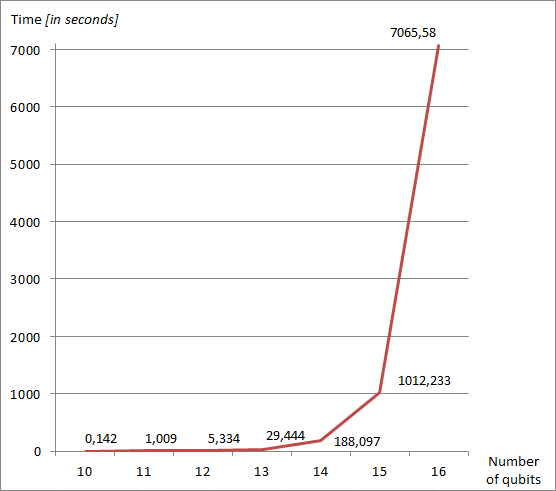
\includegraphics[width=10cm]{18_2012_1.png}
  \label{lf1}
  \caption{Increase of processing time of sequential algorithm on the Intel Xeon E7-4860  processor during the simulation of the quantum computer with deferent size of quantum register}
\end{figure}

During the analysis, the Olib library was used, which supports parallel computing. Its results in comparison with the Python programming language and NumPy module, which support only sequential operations, is shown in the Fig. \ref{lf6}

\begin{figure}
  \centering
  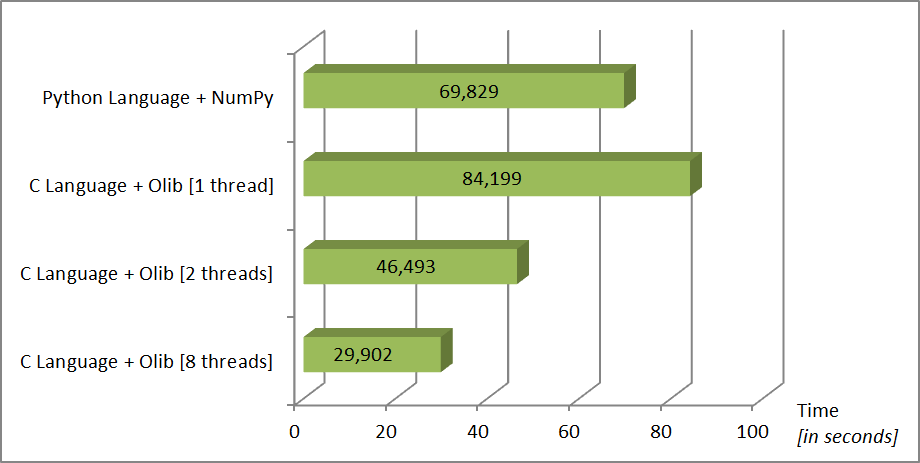
\includegraphics[width=10cm]{18_2012_6.png}
\label{lf6}
\caption{Comparison of Olib library performance with parallel processing and the NumPy (test for 14 qubits and processor Intel Core i7 920)}
\end{figure}

\subsection*{More on Olib}

Olib (\url{http://www.goldbach.pl/olib/}) is written primarily for Linux OS. In other systems (eg. Windows, BSD, Solaris) minor compatibility issues with the code may occur. Library implements efficient methods, which can be divided into following groups:

\begin{itemize}
  \item Linear algebra
  \item Discrete Mathematics
  \item Cryptography
  \item Numerical methods
  \item Artificial intelligence
\end{itemize}

Olib was optimized for several computing architectures. In one program, the programmer can combine both functions using multi-core processors and those which support graphic accelerators. The project is rather new and may not have very large set of possibilities in comparison with some other software of this type, which was developed for many years. But in many cases very good results can be achieved with it --- especially when a programmable graphic accelerator is available, or a multi-core processor, as in our case. Olib is licensed under GPL v.2 license or higher.

\subsection*{Implementation and result}

Performance tests were carried out on four different equipment platforms based on Intel Core 2 Quad Q8200 processor, Intel Core i5-2400, Intel Core i7 920 processor and the system which consists of four Intel Xeon E7-4860 processors.

\begin{figure}
  \centering
  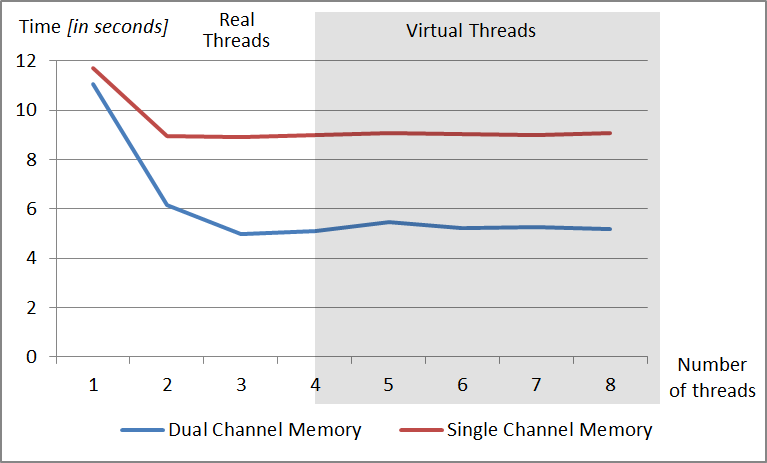
\includegraphics[width=10cm]{18_2012_2b.png}
  \label{lf2}
  \caption{Decrease of time of register simulation which consists of 13 qubits when different threads on the processor Intel Core i5-2400 and single channel memory and dual-channel memory DDR3 are used}
\end{figure}

The Fig. \ref{lf2} presents the results of the simulation of the quantum register which consists of 13 qubits and Intel Core i5-2400 processor. The minimum of 1,5 GB of free random access memory (RAM) is necessary to perform this kind of simulation. There were noticeable changes in performance when the single channel memory was used in comparison to the dual-channel DDR3 memory. Memory in the dual-channel mode reaches 21,2 GB/s maximum throughput thanks to the frequency of 1333 MHz. In the single channel mode you can reach only 10,6 GB/s. Difference in the transfer of the random-access memory has an important impact on the minimum time execution of the algorithm, which for the dual-channel memory is 5,107 seconds and for the single channel memory is 8,916 seconds.

No acceleration was noticed on older Intel Core 2 Quad Q8400 processor despite  parallel programming was used. Tested platform used single-channel memory with 10,6 GB/s capacity  but processor Core 2 Quad in comparison to the modern processors Core i5/i7 and Xeon doesn't have integrated DDR3 memory controller and that probably significantly slows down the communication process when the algorithm is processed. Results for Intel Core 2 Quad processor are shown in the Fig. \ref{lf5}

\begin{figure}
  \centering
  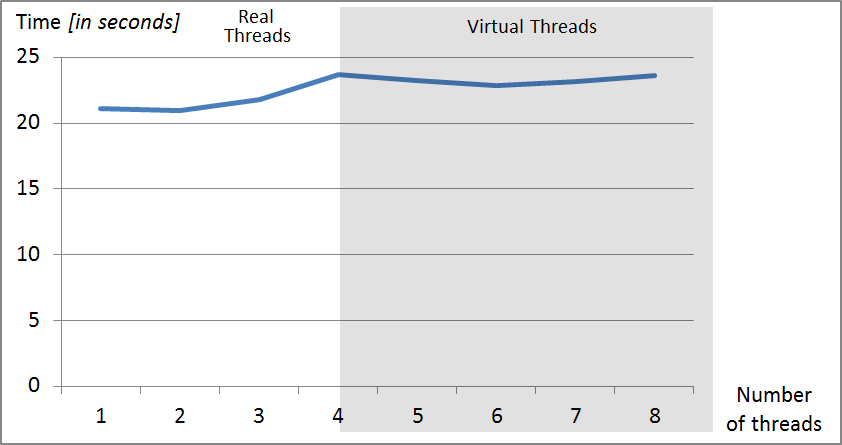
\includegraphics[width=10cm]{18_2012_5b.png}
  \label{lf5}
  \caption{Decrease of time of register simulation which consists of 13 qubits when used different threads on the processor Intel Core 2 Quad Q8400}
\end{figure}

Another tested platform is based on Intel Core i7 920 processor (fig. \ref{lf4}). It uses tri-channel DDR3 1066 MHz memory with total capacity of 25,6 GB/s. In this case, a speedup is noticeable not only for four physical cores but also after using eight threads supported by Hyper-Threading Technology. By using four threads the execution time of the algorithm is 31,049 seconds and for eight threads, with support of HT Technology it decreases to 29,902 seconds. Some tests were also carried out for eight threads on Intel Core 2 Quad Q8400 (Fig. \ref{lf5}) and Intel i5-2400 (Fig. \ref{lf2}) processors despite they have only four cores without support of HT Technology. However, it can be noticed that increase of quantity of threads without HT technology has only negative influence on the capacity because system planner must allocate excess threads to less number of processors. Additional treads which exceed physical quantity of arithmetic and logical units and can be operated by HT Technology (if available) were indicated in the diagram as Virtual Threads.

\begin{figure}
  \centering
  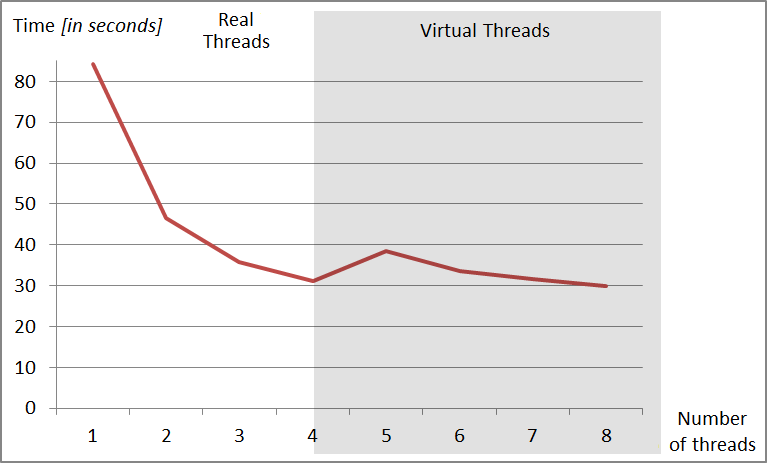
\includegraphics[width=10cm]{18_2012_4b.png}
  \label{lf4}
  \caption{Decrease of time of register simulation which consists of 14 qubits when used different threads on the processor Intel Core i7 920}
\end{figure}

The most advanced tested platform is based on four Intel Xeon E7-4860 processors. These processors support HT Technology which gives total of 80 threads in the system. However the best performance result of 384,308 is reached for 30 threads. It would take 7065,580 seconds, the usual program which is activated in sequential mode to run on this platform and it means a speedup of about 18,385. Reduction of the execution time thanks to applying many threads is show in the Fig. \ref{lf3}. This platform had physically 256 GB of DDR3 memory which enabled performing simulation of the system consisted of 16 qubits--in this case the program allocated 96 GB of memory.

\begin{figure}
  \centering
  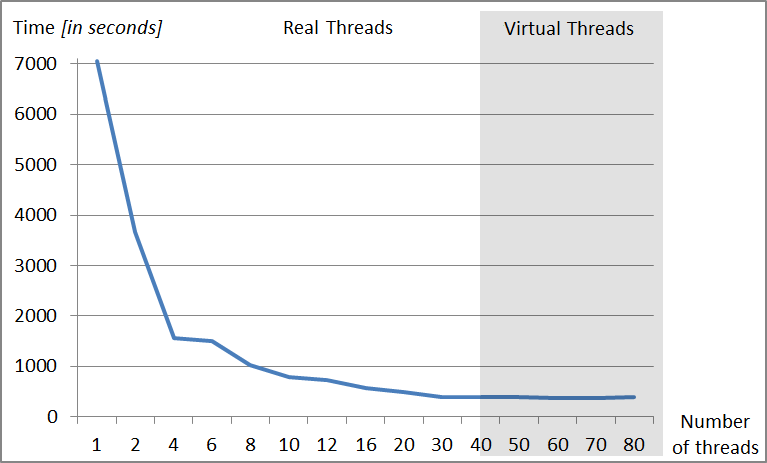
\includegraphics[width=10cm]{18_2012_3b.png}
\label{lf3}
\caption{Decrease of time of register simulation consisting of 16 qubits during using different quantity of threads on the platform which consists of four  Intel Xeon E7-4860 processors}
\end{figure}

\subsection*{Conclusion}

The possibility of simulation of the Grover's algorithm is shown. An increase of performance is noticeable on the modern parallel architectures. Usage of graphic accelerators for simulation of quantum machines can be also a very promising idea. As graphic processors handle very well typical matrices and vectors operations, so this technology can be an interesting prospect.

\begin{thebibliography}{9}
  \bibitem {l1} B. W. Kernighan, D. M. Ritchie, The C Programming Language, Prentice Hall, Inc, 1988.
  \bibitem {l2} S. Dasgupta, C. Papadimitriou, U. Vazirani, Algorytmy, Wydawnictwo Naukowe PWN, 2010.
  \bibitem {l3} Z. Czech, Wprowadzenie do obliczen rownoleglych, Wydawnictwo Naukowe PWN, 2010.
  \bibitem {l4} M. Hirvensalo, Algorytmy kwantowe, WSAP, 2010.
  \bibitem {l5} Michel Le Bellac, Wstep do informatyki kwantowej, Wydawnictwo Naukowe PWN, 2012.
  \bibitem {l6} K. Giaro, M. Kaminski, Wprowadzenie do algorytmow kwantowych, EXIT, 2003.
\end{thebibliography}


\end{document}




